\documentclass[11pt,a4paper,oneside]{article}
\usepackage[utf8]{inputenc}
\usepackage[french]{babel}
\usepackage[T1]{fontenc}
\usepackage{graphicx}
\usepackage{charter}
\usepackage{hyperref}
\usepackage{listings}
\usepackage[left=2cm,right=2cm,top=2cm,bottom=2cm]{geometry}
\author{Mylann Dupuy}
\title{Rapport de stage --  \\ Powered by \LaTeX}
\date{10 Fevrier 2017}
\begin{document}
\maketitle
\newpage
\tableofcontents
\newpage
\section{Contexte}
Le centre Jean Bernard / Clinique Victor Hugo voudrait mettre un nouveau système de déploiement pour installer et/ou mettre à jour les logiciels existants.

\section{Objectif(s)}
L'objectif est de déployer les logiciels utilisés couramment et de les mettre à jour. Le système doit fonctionner avant la fin du stage. 

\subsection{Cahier des charges}
Il fallait déployé l'ensemble des postes sur les réseaux du Centre sans que cela dérange les utilisateurs, il fallait donc mettre ne place un système de déploiement pour mettre à jour ou installer des logiciels manquants sur les postes sans déranger l'utilisateur.\\ \\
\textbf{Voici les logiciels à déployer :}\\

\begin{itemize}
	\item Adobe Flash Player 24
	\item Adobe Reader DC
	\item Java 8 Update xx
	\item Mozilla Firefox
	\item Mozilla Thunderbird
	\item PDFCreator
	\item 7-Zip
\end{itemize}

\begin{center}
\textbf{Tout les logiciels doivent êtres installés avec des paramètres spécifiques !}
\end{center}
\subsection{Contraintes}
Lors du déploiement, les postes sont constamment utilisé par le personnel du centre. Pour pouvoir intervenir, il faut appelé la personne présente sur le poste et intervenir à distance avec \textbf{TightVNC}.

\subsection{Matériels disponible}
\begin{itemize}
	\item \textbf{1 Ordinateur} pour administrer et surveiller OCS.
	\item \textbf{1 Serveur virtuel} sous \textbf{Debian 8.7}.
	\item \textbf{1 Serveur de stockage}  pour l'accès aux exécutables prévus pour les scripts. 
\end{itemize}
\newpage

\section{Solutions}
\subsection{Comparaison}
En cherchant sur Internet et aussi avec mes connaissances personnelles, j'ai recensé 4 solutions de déploiement mais dans notre contexte, il y a 2 solutions qui seront comparées car les 2 autres ne sont plus à jour. Il s'agissait de \textbf{WSUS Package Publisher} et de \textbf{Local Update Publisher} \\ \\
%%%%%%%%%%%%%%%%%%%%%%%%%%%%%%%%%%%%%%%%%%%%%%%%%%%%%%%%%%%%%%%%%%%%%%%%%%%%%%%%%%%%%%%%%%%%%%%%%%%%%%%%%%%%%%%
\begin{tabular}{|p{3.1cm}|p{6.5cm}|p{6.5cm}|}
	\hline
	\centering Solutions : & \centering Avantages : & Inconvénients : \\
	\hline
	%%%%%%%%%%%%%%%%%%%%%%%%%%%%%%%%%%%%%%%%%%%%%%%%%%%%%%%%%%%%%%%%%%%%%%%%%%%%%%%%%%%%%%%%%%%%%%%%%%%%%%%%%%%
	\centering OCS Inventory NG  & \begin{itemize}
							\item Faible utilisation de la bande passante 
							\item Plugins pour GLPI							
							\item Supervision des logiciels installé
							\item Logiciel libre disponible sous Windows Server / Client
							\item Inventaire complet des postes							
						\end{itemize} & \begin{itemize}
												\item Wiki non à jour  
												\item Paquets Debian en version 2.0.5																			\end{itemize} \\
	\hline
	%%%%%%%%%%%%%%%%%%%%%%%%%%%%%%%%%%%%%%%%%%%%%%%%%%%%%%%%%%%%%%%%%%%%%%%%%%%%%%%%%%%%%%%%%%%%%%%%%%%%%%%%%%%
	\centering WAPT  & \begin{itemize}
							\item Automatisation d'installation, MAJ et suppressions logiciels 
							\item Centralisation graphique du déploiement
							\item Facilité pour les MAJ 
							\item Gestion des dépendances
							\item Logiciel libre													
						\end{itemize} & \begin{itemize}
												\item Configuration à faire pour faire cohabiter WSUS et WAPT 
												\item Packages propre à WAPT (.wapt)
												\item Suite Microsoft Office non Disponible
												\item Supervision des logiciels installé
												\item Création de paquets + ou - complexe
												\item Certains logiciels ne sont plus à jour			
										\end{itemize} \\
	\hline	
\end{tabular}
%%%%%%%%%%%%%%%%%%%%%%%%%%%%%%%%%%%%%%%%%%%%%%%%%%%%%%%%%%%%%%%%%%%%%%%%%%%%%%%%%%%%%%%%%%%%%%%%%%%%%%%%%%%%%%
\\ \\
Nous avons décidés de mettre en place \textbf{OCS Inventory NG 2.3} (cf.Références) car les logiciels qui doivent être déployer seront facilement mis à jour contrairement à WAPT qui à certains logiciels non à jour voir même abandonner.

\subsection{Mise en \oe{}uvre}
\subsubsection{Avant de commencer} 
Nous avons créer une machine virtuelle sous Hyper-V (cf.Références) en lui mettant comme ressources :\\ \begin{itemize}
				\item 1 image ISO de Debian 8.7
				\item 4 Go de mémoire vive
				\item 1 C{\oe}ur du processeur
				\item 50 Go d'espace disque
				\item 1 connexion au réseau CJB	
\end{itemize} 

\begin{center}
\textbf{Cette configuration est hébergée sur le Poste de M.Deshayes}
\end{center}
\newpage
\subsubsection{Installation}
Lors de l'installation, j'ai tout laissé par défaut sauf le proxy qui à été renseigné. Suite à l'installation, j'ai eu à installer \textbf{openssh-server} pour tout faire via \textbf{PuTTY}.\\

Depuis SSH, il fallait installer un serveur Web, un serveur BDD, PHP, Perl et leurs modules (\textbf{apache2, mylsql-server, php5, perl, libxml-simple-perl, libcompress-zlib-perl, libdbi-perl libdbd-mysql-perl,libapache-dbi-perl, libnet-ip-perl, libsoap-lite-perl}).\\ \\
Pour les modules Perl en cas de problèmes de paquets, il faut les télécharger et les installer à la main depuis ce site \url{http://search.cpan.org/} 
S'il manque des paquets, le script d'installation d'OCS Inventory les installera mais dans notre cas, on est derrière un proxy donc vaut mieux tout installer avant. \\

Pour installer OCS Inventory NG, j'ai utilisé l'archive qui était sur le site via  et la documentation non à jour (cf.Références).
\newpage
\section{Déploiement}
\subsection{Principe de fonctionnement}
\begin{figure}[hbtp]
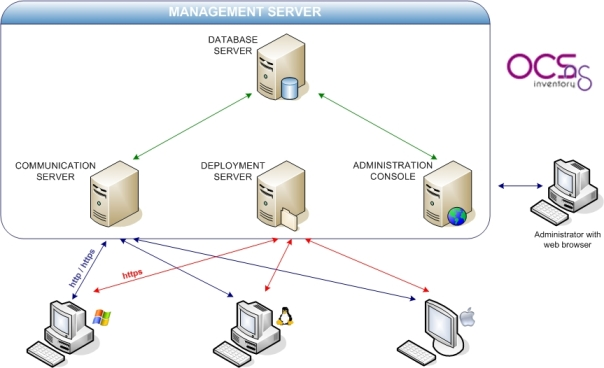
\includegraphics[scale=0.8]{../../../Downloads/deploy.jpg}
\caption{Schéma de déploiement}
\end{figure}
L'architecture reste simple à mettre en place, dans l'environnement actuel nous avons tout mis sur le même serveur.
\subsection{Outil de déploiement}
\begin{figure}[hbtp]
\centering
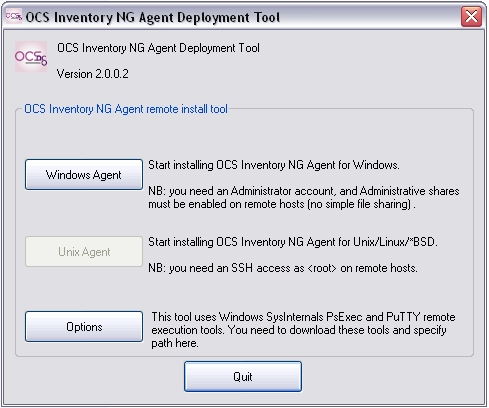
\includegraphics[scale=0.5]{../../../Pictures/Script/1.jpg}
\caption{Etape 1 - Écran de démarrage}
\end{figure}
Avant de faire le déploiement de logiciels sur le réseau, il faut installer l'agent OCS sur les postes Clients avec \textbf{OCS Inventory NG Agent Deployment Tool} puis aussi vérifier si les partages administratifs (C\$) sont bien activés. Pour ce faire, il faut faire \textbackslash\textbackslash 192.168.x.x\textbackslash C\$
 puis passer à \textbf{l'étape 2}. Si ça fonctionne pas, allez dans le Pare-Feu et autorisez le \textbf{"Partage de Fichiers et d'imprimante"}.
\newpage

\begin{figure}[hbtp]
  \centering
  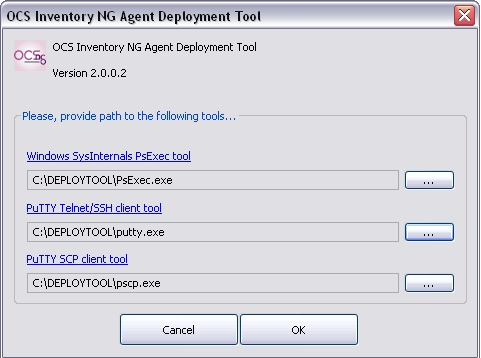
\includegraphics[scale=0.5]{../../../Pictures/Script/2.jpg}
  \caption{Etape 2 - La configuration de l'outil de déploiement}
\end{figure} 
Dans notre cas, il faut déployer l'agent sur les postes Clients mais pour ce faire, il faut utilisé le module PSEXEC (cf.Annexes) depuis le poste qui va déployer l'agent OCS. Il suffit de mettre le répertoire exacte du module précédemment télécharger depuis le site dans les options d'OCS Inventory NG Agent Deployment Tool. Quand c'est fait, il faut passer à \textbf{l'étape 3}. \\

\begin{figure}[hbtp]
 \centering
 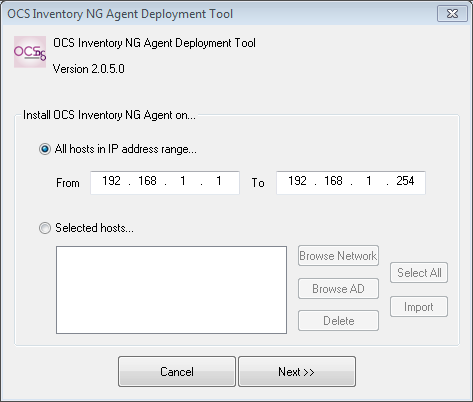
\includegraphics[scale=0.7]{../../../Pictures/Script/3.png}
 \caption{Etape 3 - La sélection des postes}
 \end{figure}
  
\textbf{l'étape 3} consiste à définir une plage IP  ou à sélectionner le(s) Poste(s) qui auront l'agent OCS. Dans notre cas, on avait défini une plage IP sur l'ensemble du réseau CJB. Après la selection des postes, on passe à \textbf{l'étape 4}.
\newpage

\begin{figure}[hbtp]
\centering
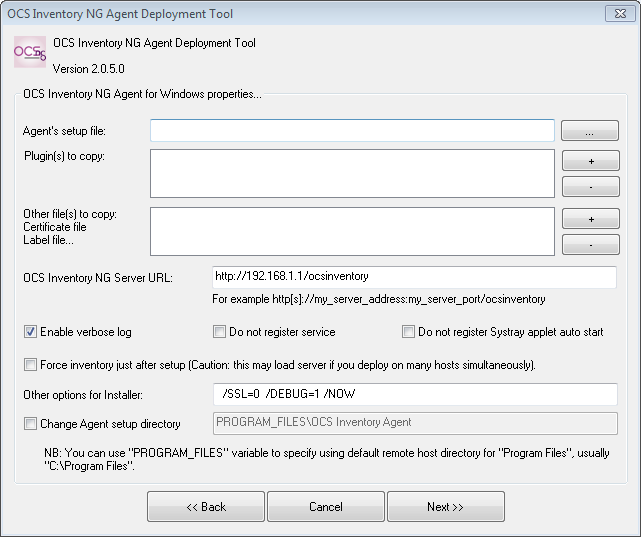
\includegraphics[scale=0.7]{../../../Pictures/Script/4.png}
\caption{Etape 4 - Les paramètres de l'agent OCS}
\end{figure}

C'est à partir de là qu'on va faire la configuration de l'agent OCS qui sera mis en place lors du déploiement.  
\begin{enumerate}
\item Il faut lui donner le répertoire où se trouve le fichier d'installation de l'agent.
\item Les plugins ou fichier à copier sur le Poste Client.
\item Le certificat du serveur si SSL est activé sur le serveur OCS.
\item L'adresse URL du serveur OCS.
\item Activer les options pour l'agent OCS (Logs, Ne pas enregistrer en tant que service, Ne pas mettre l'icône dans la barre de notifications au démarrage du Poste, Forcer l'inventaire après l'installation).
\item Les options spécifiques qu'on veut mettre. Les options choisies au dessus sont écrites dans cet encadrement.
\item Le répertoire d'installation pour l'agent OCS sur le(s) Poste(s) Client(s).
\end{enumerate}
Quand cette étape est faite en ayant bien vérifier avant, on passe à \textbf{l'étape 5} qui terminera les étapes de configuration de l'agent.
\newpage
\begin{figure}[hbtp]
\centering
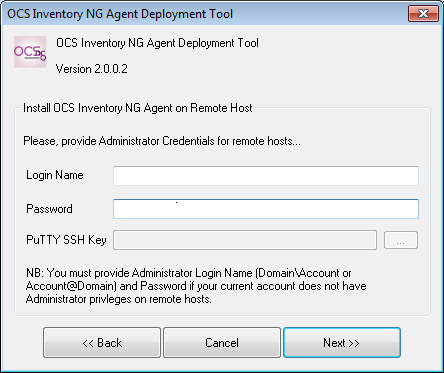
\includegraphics[scale=0.9]{../../../Pictures/Script/5.png}
\caption{Etape 5 - L'authentification}
\end{figure}

Pour permettre le déploiement de l'agent OCS SANS déranger les utilisateurs ni en intervenant sur les postes clients, il faut renseigner les informations de connexion du compte "Administrateur" du domaine pour les postes WINDOWS. Si les informations sont exactes, on lance le déploiement à l'étape 6.

\begin{figure}[hbtp]
\centering
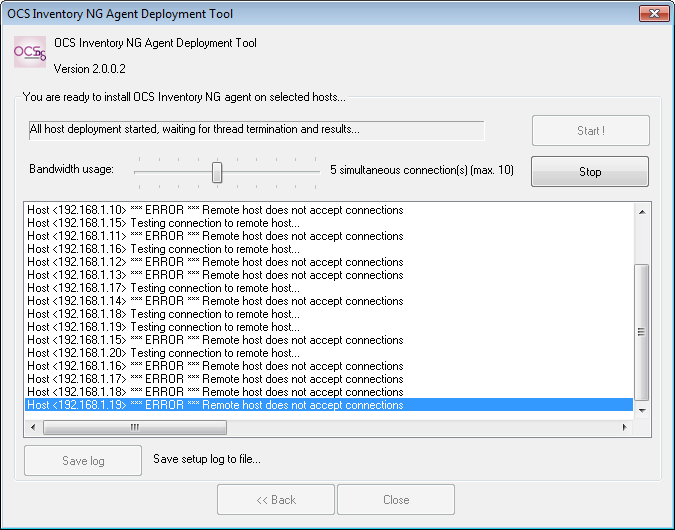
\includegraphics[scale=0.6]{../../../Pictures/Script/6.png}
\caption{Etape 6 - Log de déploiement}
\end{figure}

Après avoir tout bien fait, il suffit de lancer le déploiement pour qu'il installe l'agent OCS sur les postes Clients. L'outil de déploiement peut déployer les postes Clients 1 par 1 ou peut faire 10 connexions simultanées, c'est-à-dire qu'il va faire l'operation sur 10 postes maximum. \\ 
\textbf{ATTENTION ! En changeant le nombre de connexion simultanées, on augmente la charge du CPU.}
\newpage
\subsection{Interface Web OCS Inventory}
Lors que l'agent est bien installé sur les postes Clients, il doivent faire l'inventaire complet de la machine et envoyer automatiquement l'inventaire au serveur. Suite à ça, on peut se faire une idée sur les logiciels qu'on doit déployer ou non. \\

En arrivant sur l'écran d'inventaire, on remarque les différentes informations sur les postes Clients (TAG, Dernier Inventaire, Le nom de l'ordinateur, L'utilisateur actuel, OS, Fréquences RAM / CPU) qui sont automatiquement inventoriés selon la configuration faite depuis le serveur.
\subsection{Scripts}

OCS Inventory peut déployer des paquets SEULEMENT s'ils sont en ".zip" ou ".tar.gz" donc avant de déployer un paquets, on va créer un script qui va lancer les installations des logiciels de manière silencieuse et avec des paramètres spécifiques.
\\	
Ce sont des scripts Batch qui ont été réalisés pour CHACUN des logiciels. Le contenu est quasiement le même sauf pour la désinstallation et l'installation qui demandent des options spécifiques (No reboot, silencieux, aucune interaction avec l'utilisateur).
\\
Lors de l'installation des logiciels, il ne faut pas que cela perturbe le travail de l'utilisateur donc il faut AUCUNE interaction donc pas de boîte de dialogue ni d'autorisation utilisateur ni de "Pop-Up" et SURTOUT PAS de redémarrage surtout dans ce contexte.
\newpage
On va prendre l'exemple de Mozilla Firefox avec le code disponible :
\\
\textbf{Voir en annexes les différentes commandes}
  

\begin{lstlisting}[language=C]
@echo off
1	runas /profile /user:Administrateur install.bat < pass.txt
	
3	sc config UI0Detect start= disabled
4	sc stop UI0Detect

6	"C:\Program Files (x86)\Mozilla Maintenance Service\Uninstall.exe" 
7	/verysilent /SUPPRESSMSGBOXES /NORESTART
	
9	"C:\Program Files (x86)\Mozilla Firefox\uninstall\helper.exe" 
10	/verysilent /SUPPRESSMSGBOXES /NORESTART
	
11	"C:\Program Files\Mozilla Firefox\uninstall\helper.exe" 
12	/verysilent /SUPPRESSMSGBOXES /NORESTART	

14	"\\ficserv\allusers\Logiciels\firefox\Firefox Setup 51.0.1.exe" 
15	/INI=\\ficserv\allusers\Logiciels\firefox\config.ini 
16	/verysilent /SUPPRESSMSGBOXES /NORESTART
	
18	powershell -executionpolicy Bypass -file "\\192.168.10.28\allusers
19	\Logiciels\01 - Install Mat\Script\Firefox\Firefox.ps1"	
	
21	"%ProgramFiles%\Mozilla Firefox\uninstall\helper.exe" 
22	/SetAsDefaultAppUser
	
goto end
:end	
\end{lstlisting}
\begin{itemize}
	\item Ligne 1 : Avec la commande \textbf{RUNAS}, on se connecte en tant qu'Administrateur lors de l'exécution de ce script et pour pas à avoir à taper le mot de passe, le script utilise le fichier "pass.txt" qui contient le mot de passe en clair.
	\item Ligne 3 - 4: Il faut désactiver le services U10Detect (cf.Références) pour que rien n'apparaisse à l'écran car  même en voulant faire une installation silencieuse, il y a toujours des programme qui se lance mais sans option silencieuse donc vaut mieux le désactiver. Après l'avoir désactiver, il faut arrêter le service en utilisant toujours SC (cf.Références). 
	\item Ligne 6 - 12 : Répertoire où se trouve le programme de désinstallation de Mozilla Firefox et de Mozilla Maintenance Service.
	\item Ligne 14 - 16 : Répertoire où se trouve le programme de d'installation de Mozilla Firefox en utilisant son fichier de configuration (Répertoire d'installation du Poste Client, Mettre ou non raccourcis sur le bureau ou la barre de lancement ou dans le menu démarrer, la désactivation du Maintenance Service). Faire l'installation silencieuse, supprimer tout les messages qui peuvent apparaitre et ne pas redémarrer
	\item Ligne 18 - 19 : Récupérer une icône car l'ancienne ne fonctionnera plu (Cf.Problèmes rencontrés) en utilisant un script maison en PowerShell.
	\item Ligne 21 - 22 : Faire de Mozilla Firefox le navigateur par défaut avec le paramètre
\end{itemize}
\newpage
\subsection{Déploiement}
\subsubsection{Création}
Après que le script soit fait, il reste à créer l'archive en ".zip" avec le fichier ".txt" qui contient le mot de passe et le script Batch. En général, l'archive fait moins de 5 Kilo-Octet. Quand l'archive à bien été faite, il y a plu qu'a créer la fiche du déploiement en se connectant sur l'interface Web d'OCS et aller dans "Deployment" puis "Build"
\\
\begin{figure}[hbtp]
\centering
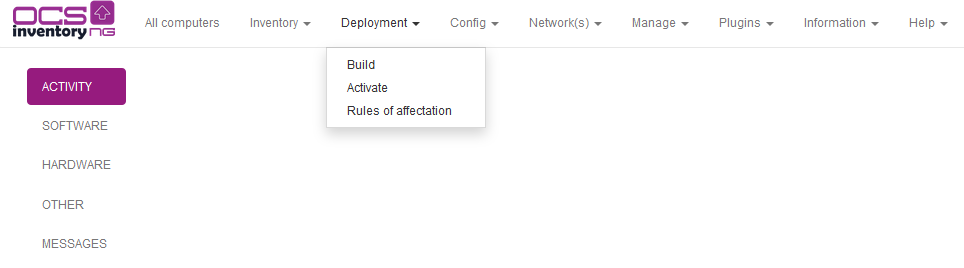
\includegraphics[scale=0.7]{../../../Pictures/Script/Deploiement1.PNG}
\caption{Accès Creation Déploiement}
\end{figure}

Après avoir cliqué dessus, la page "Package Builder" s'ouvre en y montrant un liste à remplir

Il faut renseigner le nom, la description du paquet, sur quel OS faut l'installer, le protocole (dans mon cas, j'ai pas mis en HTTPS), la priorité du déploiement (Chiffre le + haut est prioritaire), le fichier à déployer (mettre l'archive précédemment crée), executer ou non une commande à l'extraction du package donc la c'est le nom du script Batch. Le reste n'est pas à renseigner car on a pas de serveur de redistribution et on veut pas que l'utilisateur soit averti.
\begin{figure}[hbtp]
\centering
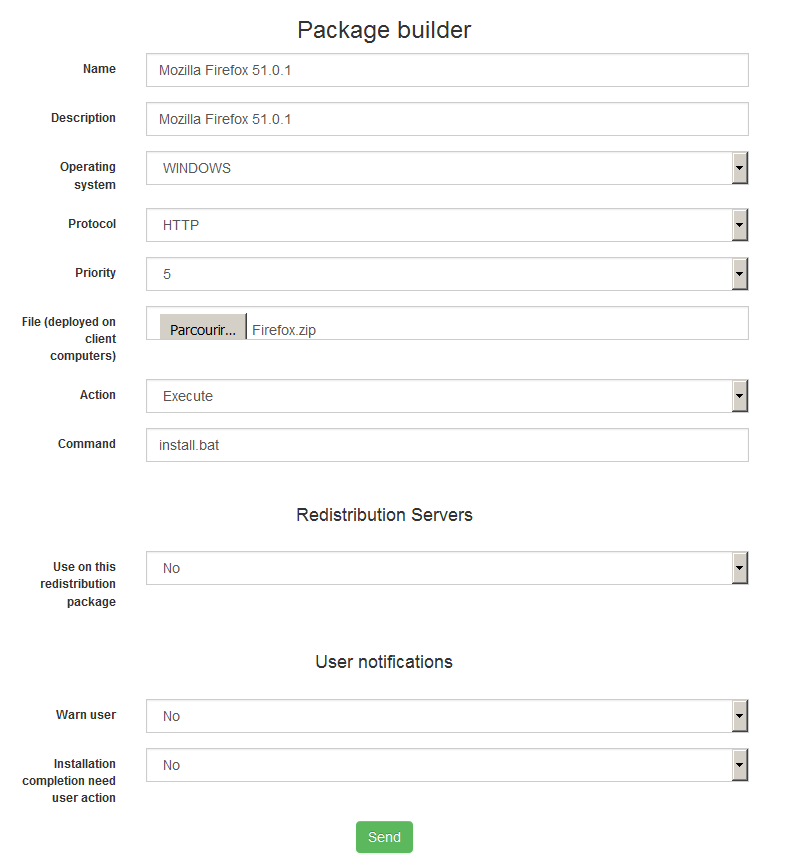
\includegraphics[scale=0.4]{../../../Pictures/Script/Deploiement2.PNG}
\caption{Information Déploiement}
\end{figure}
\newpage

La page finale de création du paquet montre le poids du paquet, le nombre de fragment du paquets pour pas saturer le réseau lors du déploiement de gros paquet (c'est pas notre cas) et le temps estimé pour le déploiement (qui affiche souvent rien)

\begin{figure}[hbtp]
\centering
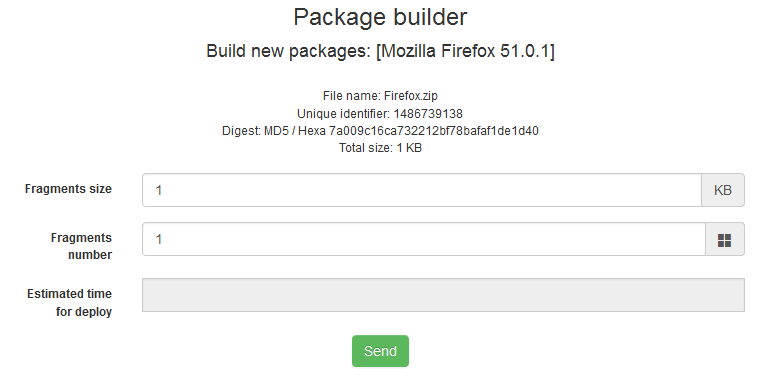
\includegraphics[scale=0.6]{../../../Pictures/Script/Deploiement3.PNG}
\caption{Résumé de création}
\end{figure}

Dès que la confirmation apparait, cela veut dire que le paquets est bien créer dans le répertoire "/var/lib/ocsinventory-reports/download/......". On peut voir que tout les paquets de déploiement crées appartienne à "www-data"

\begin{figure}[hbtp]
\centering
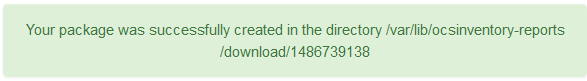
\includegraphics[scale=0.6]{../../../Pictures/Script/Deploiement4.PNG}
\caption{Confirmation de Création du paquets}
\end{figure}

\begin{figure}[hbtp]
\centering
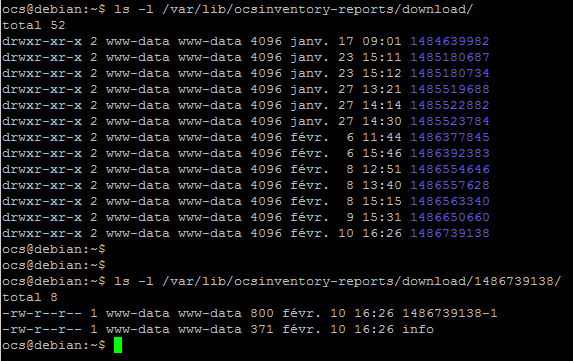
\includegraphics[scale=0.7]{../../../Pictures/Script/Deploiement5.PNG}
\caption{Résultat coté serveur}
\end{figure}
\newpage
\subsubsection{Activation}

Après avoir eu la confirmation de la création du paquet, il reste à l'activer pour pouvoir le déployer sur les postes. Et pour ce faire, il faut faire la même opération de tout à l'heure mais cette fois, il faut cliquer sur "Activate"

\begin{figure}[hbtp]
\centering
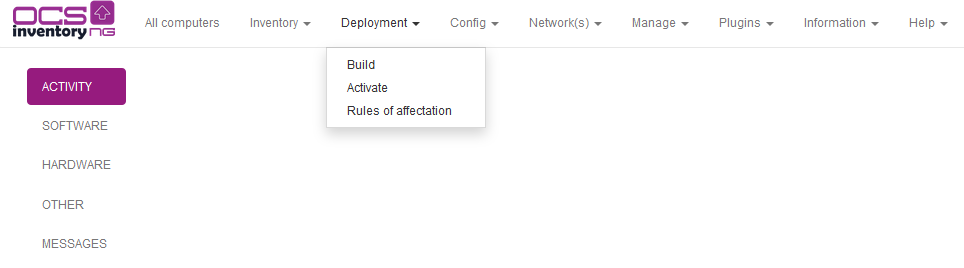
\includegraphics[scale=0.7]{../../../Pictures/Script/Deploiement1.PNG}
\caption{Accès Activation Paquet}
\end{figure}

Après avoir cliqué dessus, la page "Package Activation" s'ouvre en y montrant la liste des paquets disponibles pour le déploiement

\begin{figure}[hbtp]
\centering
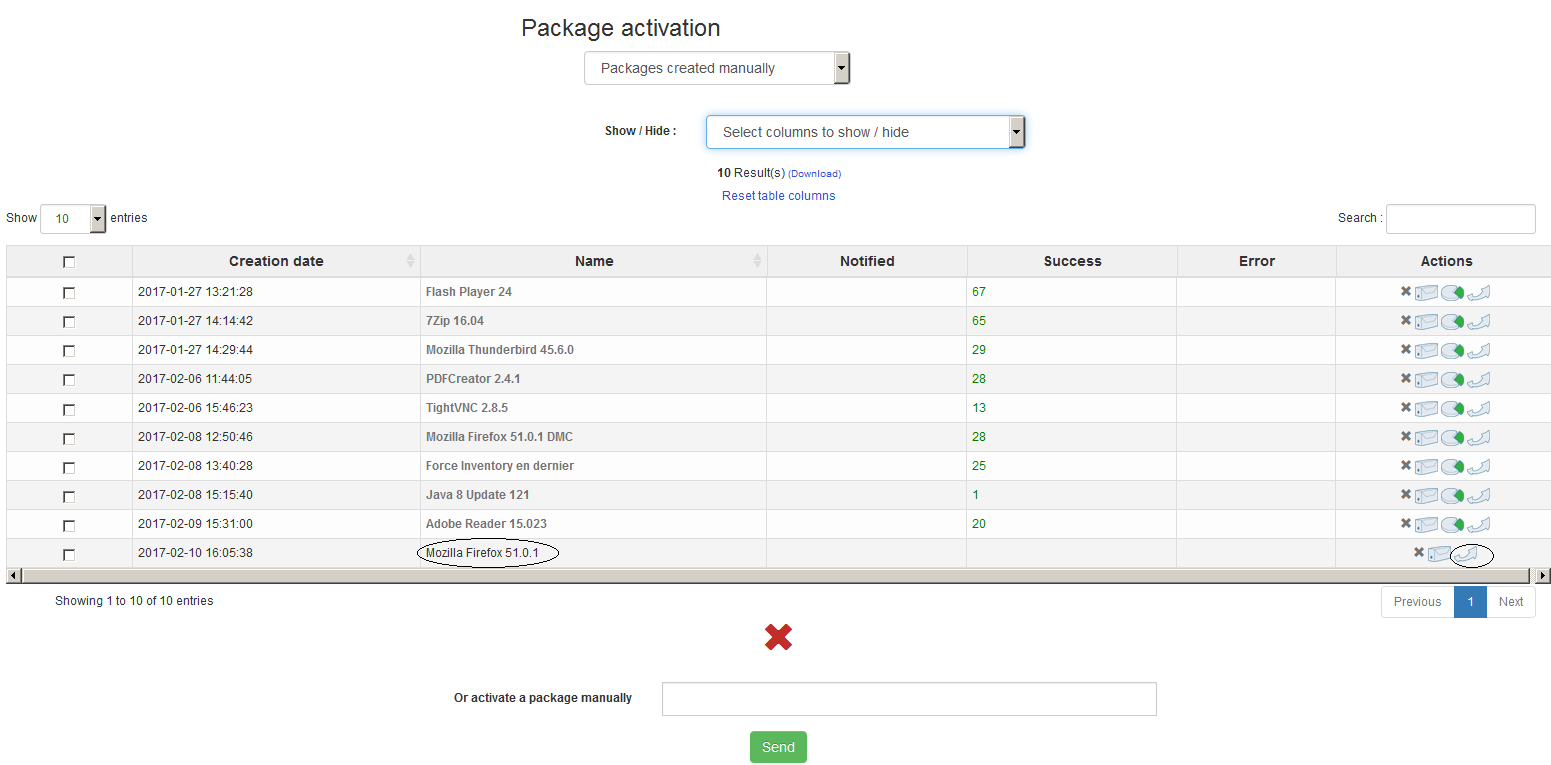
\includegraphics[scale=0.4]{../../../Pictures/Script/Activation2.PNG}
\caption{Accès Activation Paquet}
\end{figure}
 
Par rapport aux autres paquets déjà déployés, celui qu'on à crée est affiché différemment, il apparait en "Noir" alors que les autres apparaissent en "Gris" car ils ont été activés et pas le nôtre. Pour ce faire, il faut sur la "Flèche en double sens" à droite de l'écran. Suite à ça, il demande confirmation pour l'activation et ensuite notre paquet devient "Grisé" comme les autres.
\newpage

\section{Résultat Final}
Lorsque le déploiement est fini, il suffit de regarder dans la liste des programmes installés directement sur OCS ou de voir sur le poste client. Le déploiement peut rencontré des problèmes donc il faut pas hésité à aller voir dans \textbf{l'Observateur d'Evenements} car souvent, c'est un problème dû à Windows Installer qui n'a pas les droits requis pouu l'installation alors qu'on démarre le script en utilisateur "Administrateur"
\subsection{Problèmes rencontrés}
Tout au long de ce stage en mettant en place le déploiement par OCS Inventory NG, j'ai eu quelques soucis que j'ai pu résoudre mais pas tous car pour certains, il fallait intervenir sur les postes ou sinon c'était un service WINDOWS qui posait problème.
\\
\begin{itemize}
\item Windows 7 bloque le déploiement des paquets à cause d'un service de "Détection de services interactifs".
\item Mozilla Maintenance Service posait problème quand le service de "Détection de Services Interactifs" s'activer, il affichait une boite de dialogue à l'utilisateur.
\item PDFCreator mettait son imprimante par défaut mais avec un import/export du registre pendant le script, l'imprimante d'origine se remet par défaut (en pratique au bureau informatique).
\item  Adobe Reader se désinstalle mais ce réinstalle pas car il n'a pas les droits suffisants sur certains postes (MSIInstaller en cause) !!!
\item PDFCreator demande à faire redémarrer le PC.
\item L'utilisation de PSEXEC va créer un dossier utilisateur sur l'ordinateur distant... Résolu avec un script qui force le déploiement de l'inventaire OCS et supprime le dossier utilisateur (cf.Annexes).
\item Suite à la mise à jour de Firefox, les PDF s'ouvrent sur une nouvelle page au lieu d'un nouvelle onglet.
\item A la suite du déploiement, les raccourcis .URL ne pointent plu vers le navigateur. Résolu par un script Powershell (Cf.Annexes)
\end{itemize}

\section{Conclusion}
Durant les 8 semaines de stage, j'ai pu apprendre et travailler au sein d'une d'équipe sur un ensemble de postes en mettant en place un système de déploiement qui servira (ou non) au fil du temps. En cherchant des solutions de déploiement, j'ai pu connaitre autre chose qu'OCS Inventory NG (Cf.Solutions).

J'ai découvert aussi les contraintes qu'il pouvait y avoir en labo et lors d'un déploiement réel sur le réseau du centre en rencontrant des problèmes résolus ou non.
\newpage
\section{Annexes}
\subsection{Scripts}
Script avec MSIEXEC (pour les package .msi).
\begin{lstlisting}[language=C]
1 @echo off

3	runas /noprofile /user:Administrateur install.bat < pass.txt

5 Desactivation du service de Detection de services interactifs
6	sc config UI0Detect start= disabled
7	sc stop UI0Detect

9 Desinstallation de Flash Player (tous modules)
10	"\\ficserv\allusers\Logiciels\flash player\
11	uninstall_flash_player.exe" -uninstall

13 Installation de Flash Player
14	msiexec /i "\\ficserv\allusers\Logiciels\
15	flash player\install_flash_player_24_active_x.msi" /quiet /norestart
	
17	msiexec /i "\\ficserv\allusers\Logiciels\
18	flash player\install_flash_player_24_plugin.msi" /quiet /norestart

20 Fichier de Configuration d'Adobe Flash 
21	xcopy "\\ficserv\allusers\Logiciels\
22	flash player\mms.cfg" /Y C:\windows\syswow64\macromed\flash\ 

24 Reactivation du Service de Detection de services interactifs
25	sc config UI0Detect start= demand
26	sc stop UI0Detect

28 goto end
29 :end
\end{lstlisting}

Le script est à peu près le même que pour celui de Mozilla Firefox crée précédemment sauf que cette fois, il s'agit d'un package .MSI.\\
En détail sur les lignes de désinstallation et d'installation : (Cf.Annexes) \\
\begin{itemize}
\item Ligne 10 : L'exécutable .exe permet de supprimer TOUTES les versions d'Adobe Flash Player présente sur 			l'ordinateur de manière silencieuse vu qu'on lui ajoute le paramètre "-uninstall" \\

\item Ligne 13 - 14 : Le package .MSI démarrera en mode silencieux et sans redémarrer comme indiquer avec les paramètres "/quiet" et "/norestart"
\end{itemize}
\newpage
Script PowerShell pour changer les raccourcis Internet des postes clients

\begin{lstlisting}[language=C]

$ProfilesDirectory = (get-itemproperty -Path "HKLM:\SOFTWARE\Microsoft\Windows NT\
CurrentVersion\ProfileList" -Name ProfilesDirectory).ProfilesDirectory

Get-ChildItem -Path $ProfilesDirectory -filter DMC.lnk 
-recurse -Force | foreach ($_) {Remove-Item $_.FullName ; Copy-Item -Path
 \\ficserv\allusers\dmc\DMC.lnk -Destination $_.DirectoryName}

Stop-Process -Name powershell

\end{lstlisting}
\textbf{Commentaires :}\\
\begin{itemize}
\item \textbf{Variable \$ProfileDirectory :} Récupère à partir du registre, les répertoires Utilisateurs existants dans le Disque Local C: 
\item \textbf{Variable Get-ChildItem :} Depuis la variable \$ProfilesDirectory, le script va filtré dans tout les dossiers utilisateur l'icône "DMC.lnk" en la supprimant (si trouvé) et en copiant depuis le serveur la nouvelle icône fonctionnelle 
\end{itemize}

\subsection{Définitions}
\textbf{Microsoft Hyper-V :} Virtualisation de machines en ayant le service d'installer sur un Windows 8.x minimum, fonctionne à peu près comme VirtualBox
\\ \\
\textbf{PSEXEC :} PsExec est un outil en ligne de commande fournit dans la suite PsTools de chez Sysinternals. Il permet d’exécuter à distance des commandes, des programmes, des batches, comme si vous étiez connecté sur le serveur distant.
\\ \\
\textbf{RUNAS :} La commande RUNAS permet à un utilisateur d'exécuter des outils et des programmes spécifiques avec des autorisations différentes de celles attribuées à l'ouverture de session; par exemple, si vous désirez exécuter un programme nécessitant des droits d'Administrateur alors que vous n'êtes pas connecté en tant que tel.
\\ \\
\textbf{Commande SC :} L'utilitaire de contrôle des services SC est un puissant outil en ligne de commande permettant de gérer les services Windows. Cet outil permet également d'arrêter et de démarrer rapidement les services afin de résoudre les problèmes.
\\ \\
\textbf{U10Detect :} Active la notification des entrées utilisateur pour les services interactifs, qui active l'accès aux boîtes de dialogue créées par les services interactifs lorsqu'elles apparaissent.
\\ \\
\textbf{MSIEXEC :} La commande msiexec utilise des paramètres pour donner à MSI une partie ou l'ensemble des informations pouvant être spécifiées au sein d'une installation interactive. Cela signifie qu'un utilisateur peut créer une configuration d'installation automatique ou semi-automatique réutilisable. Les paramètres peuvent être fournis via la ligne de commande, un fichier de conversion, un fichier de réponse ou une combinaison des trois
\newpage

\section{Références}
\begin{itemize}
\item \textbf{Adobe :} \url http://www.adobe.com/fr/ 
\item \textbf{Java :} \url https://www.java.com/fr/
\item \textbf{Mozilla :} \url https://www.mozilla.org/fr/
\item \textbf{PDFCreator :} \url http://www.pdfforge.org/pdfcreator
\item \textbf{Debian 8.x :} \url https://www.debian.org/index.fr.html 
\item \textbf{OCS Inventory NG :} \url www.ocsinventory-ng.org/fr/
\item \textbf{WAPT :} \url {https://dev.tranquil.it/wiki/WAPT_-_apt-get_pour_Windows}
\item \textbf{WSUS Package Publisher :} \url https://wsuspackagepublisher.codeplex.com/
\item \textbf{Local Update Publisher :} \url http://localupdatepubl.sourceforge.net/fr/index.html
\item \textbf{Wiki d'OCS Inventory :} \url{http://wiki.ocsinventory-ng.org/index.php?title=Documentation:Server/fr}
\item \textbf{OCS Inventory NG Agent Deployment Tool :} \url http://wiki.ocsinventory-ng.org/index.php?title=Documentation:DeployTool/fr
\end{itemize}


\newpage
\end{document}